% Section 1: Introduction
% Word count target: ~900 words

\section{Introduction}
\label{sec:introduction}

Protein-protein interactions (PPIs) form the molecular foundation of cellular life. Virtually every biological process---signal transduction, immune response, metabolism, gene regulation---relies on proteins interacting with specific partners. The human interactome is estimated to contain 130,000--650,000 binary interactions~\cite{szklarczyk2021string}, with each protein engaging an average of 5--10 partners. Disease-associated mutations disproportionately affect interaction interfaces: Sahni et al.~\cite{sahni2015edgotype} demonstrated that approximately 60\% of disease mutations perturb at least one protein-protein interaction, and over 25\% result in complete loss of interactions. These findings establish PPIs as important molecular determinants of disease phenotypes and attractive therapeutic targets.

Over the past two decades, computational approaches to PPI research have primarily focused on \textit{prediction}: given protein sequences or structures, infer whether and how they interact. This prediction paradigm has produced remarkable successes. Methods like PIPR~\cite{chen2019pipr} and D-SCRIPT~\cite{sledzieski2021dscript} achieve high accuracy in predicting binary interactions from sequence alone. AlphaFold-Multimer~\cite{evans2022alphafoldmultimer} and AlphaFold 3~\cite{abramson2024alphafold3} predict the three-dimensional structures of protein complexes with unprecedented accuracy. These capabilities have accelerated interactome mapping and enabled structure-based analysis of interaction networks.

Yet a fundamental limitation constrains prediction methods: they can only describe what might happen, not create what we want to happen. For drug discovery and synthetic biology, the relevant question is not ``will these proteins interact?'' but ``how can we design proteins that interact the way we need?'' This shift from passive observation to active creation defines the emerging \textit{design paradigm}.

\subsection*{Why This Paradigm Shift Matters}

The transition from prediction to design represents more than methodological evolution---it constitutes what Thomas Kuhn termed a ``paradigm shift'' in scientific practice~\cite{kuhn1962structure}. In Kuhn's framework, paradigms define not only what questions scientists ask but what questions are considered meaningful. The prediction paradigm asks: ``What interactions exist in nature?'' The design paradigm asks: ``What interactions can we create?'' This reconceptualization opens investigation into regions of sequence-structure space that evolution never explored but that may contain superior therapeutic or industrial properties.

The practical significance is substantial. Traditional drug discovery---screening large compound libraries---identifies leads against approximately 15\% of potential targets, leaving the majority ``undruggable'' due to lack of suitable binding pockets or chemical matter. Protein-based therapeutics can engage flat protein surfaces inaccessible to small molecules, potentially expanding druggable target space several-fold. Similarly, synthetic biology currently relies on repurposing natural protein components; design capabilities would enable creation of signaling pathways and biosensors unconstrained by evolutionary history.

The economic implications are equally significant. Drug development costs, including failed candidates, are estimated at \$0.8--2.0 billion per approved therapeutic (median: \$1.3 billion) with timelines of 10--15 years~\cite{wouters2020cost}. Computational design could compress early-stage discovery from years to weeks, reducing both costs and time-to-patient. Early applications to SARS-CoV-2 demonstrated this potential: designed neutralizing proteins reached preclinical testing within 6--8 weeks rather than the years typically required for antibody development~\cite{watson2023rfdiffusion}.

\subsection*{Technological Foundations and Controversies}

This review argues that the field is undergoing a paradigm shift enabled by converging technological advances. Protein language models encode evolutionary and structural information at scale~\cite{rives2021esm1b,lin2023esm2}. Diffusion models generate novel protein structures conditioned on functional constraints~\cite{watson2023rfdiffusion,ingraham2023chroma}. Equivariant neural networks preserve geometric symmetries essential for accurate structure modeling~\cite{jing2021gvp,fuchs2020se3transformer}. Together, these technologies enable the creation of novel proteins with desired interaction properties.

However, the field is not without controversy. Critics note that success rates for de novo design remain modest (10--50\% depending on target) compared to natural protein engineering~\cite{bernett2024bias}. Questions persist about whether designed proteins will exhibit the stability, specificity, and lack of immunogenicity required for therapeutic use. Some argue that current ``design'' methods are better characterized as sophisticated optimization of natural scaffolds rather than true creation~\cite{kewalramani2023state}. This review addresses these critiques while presenting evidence that a paradigm shift, though incomplete and ongoing, represents a meaningful transformation in the field's capabilities.

The challenges are significant. Current methods struggle with dynamic interactions, multi-protein complexes, and generalization to novel targets. Evaluation remains problematic, with data leakage potentially inflating reported performance. The experimental validation bottleneck limits iterative improvement. These challenges define the research frontier that the field must address to realize the paradigm's full potential.

\subsection*{Article Structure}

This review provides a comprehensive analysis of this paradigm shift. Section~\ref{sec:prediction} examines the prediction paradigm's methods and limitations. Section~\ref{sec:design} traces the emergence of design capabilities. Section~\ref{sec:design_tasks} surveys core design tasks. Section~\ref{sec:technologies} details enabling technologies. Section~\ref{sec:challenges} discusses open challenges. Section~\ref{sec:applications} examines applications in therapeutics, synthetic biology, and basic research. Section~\ref{sec:future} offers perspectives on future directions, and Section~\ref{sec:conclusion} synthesizes key themes.

% ===== FIGURE 1: 范式转变概览图 =====
% 
% 图表类型: 双面板对比图 (Two-panel comparison diagram)
% 尺寸: 全页宽度 (single-column width for journal)
% 
% 【左面板 - 预测范式】
% 标题: "Prediction Paradigm"
% 
% 核心流程图 (从上到下的垂直流程):
% ┌─────────────────────────────────────────┐
% │         Input: Known Proteins           │
% │         (Sequences/Structures)          │
% └─────────────────┬───────────────────────┘
%                   ↓
% ┌─────────────────────────────────────────┐
% │    Computational Analysis/Prediction    │
% │    • Sequence similarity                │
% │    • Structure comparison               │
% │    • Machine learning classification    │
% │    (Methods: SVM, GNN, Transformers)    │
% └─────────────────┬───────────────────────┘
%                   ↓
% ┌─────────────────────────────────────────┐
% │    Output: Binary Classification        │
% │    "Will these proteins interact?"      │
% │    Answer: YES / NO                     │
% │    (Optional: Where? How strongly?)     │
% └─────────────────────────────────────────┘
%
% 特征标注:
% • 箭头: 灰色/蓝色
% • 问题标记: "Discovery Mode" 标签
% • 时间指示: "1980s-2020" (底部)
% • 关键词: "Understanding", "Analysis", "Classification"
%
% 【右面板 - 设计范式】
% 标题: "Design Paradigm"
%
% 核心流程图 (循环流程):
% ┌─────────────────────────────────────────┐
% │    Input: Design Goal/Target            │
% │    "What interaction do we WANT?"       │
% │    (Target structure + constraints)     │
% └─────────────────┬───────────────────────┘
%                   ↓
% ┌─────────────────────────────────────────┐
% │       Generative AI Design              │
% │    • Diffusion models (backbone)        │
% │    • Inverse folding (sequence)         │
% │    • Multi-objective optimization       │
% │    (Methods: RFdiffusion, AlphaProteo)  │
% └─────────────────┬───────────────────────┘
%                   ↓
% ┌─────────────────────────────────────────┐
% │    Output: Novel Protein Sequences      │
% │    "Here are proteins that WILL bind"   │
% │    (Candidate designs: 100s-1000s)      │
% └─────────────────┬───────────────────────┘
%                   ↓
% ┌─────────────────────────────────────────┐
% │    Validation & Iteration               │
% │    • Computational screening            │
% │    • Experimental testing               │
% │    • Feedback to improve design         │
% └─────────────────┬───────────────────────┘
%                   ↓ (loop back to top)
%
% 特征标注:
% • 箭头: 绿色/紫色
% • 循环标记: "Creative Mode" 标签
% • 时间指示: "2021-Present" (底部)
% • 关键词: "Creation", "Engineering", "Synthesis"
%
% 【中间分隔区域】
% 大箭头: 从左到右，标注 "PARADIGM SHIFT"
% 副标题: "From Analysis to Synthesis"
%
% 【底部对比表】(small table)
% ┌──────────────┬─────────────────┬──────────────────┐
% │ Aspect       │ Prediction      │ Design           │
% ├──────────────┼─────────────────┼──────────────────┤
% │ Goal         │ Understand      │ Create           │
% │ Question     │ "Will it?"      │ "How to make it?"│
% │ Output       │ Yes/No          │ New sequences    │
% │ Role of AI   │ Analyzer        │ Creator          │
% │ Key Methods  │ Classification  │ Generation       │
% └──────────────┴─────────────────┴──────────────────┘
%
% 颜色方案:
% • 背景: 白色
% • 预测范式: 蓝色系 (#4A90E2, #7BA3E2)
% • 设计范式: 绿色系 (#7ED321, #A8E6CF)
% • 箭头: 深灰色 (#4A4A4A)
% • 文字: 黑色 (#000000)
%
% 脚注: "Figure 1: The paradigm shift from prediction to design in AI-driven protein-protein interaction research. 
%        Left: The prediction paradigm analyzes existing proteins to determine interaction likelihood. 
%        Right: The design paradigm generates novel proteins with desired interaction properties."

\begin{figure}[t]
\centering
\resizebox{0.95\textwidth}{!}{%
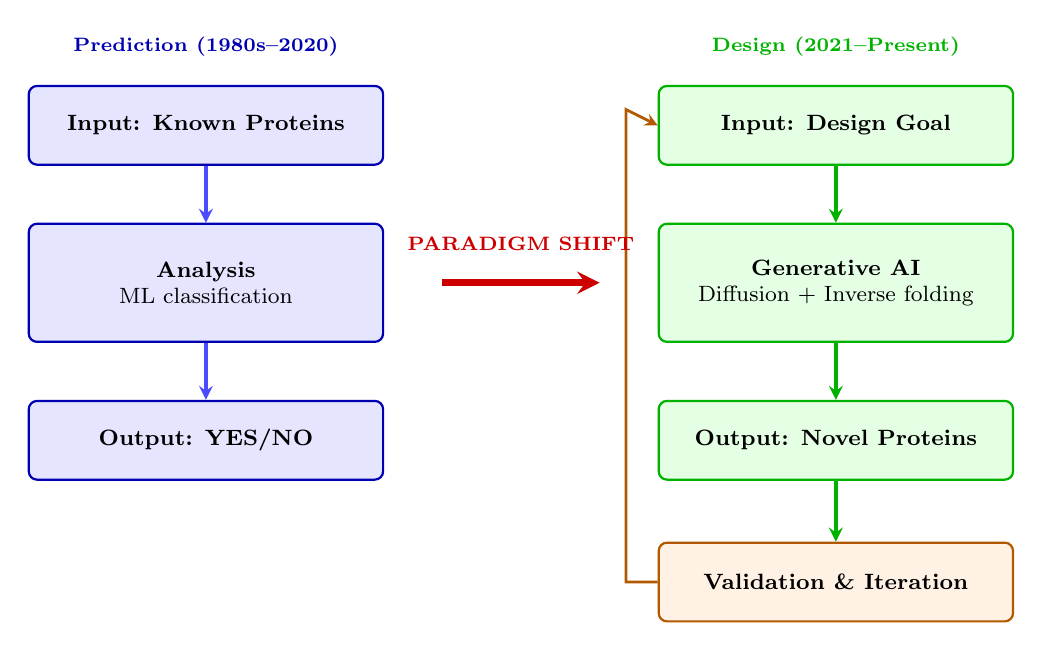
\begin{tikzpicture}[
    box/.style={rectangle, rounded corners=3pt, draw, minimum width=4.5cm, minimum height=1cm, align=center, font=\footnotesize},
    predbox/.style={box, fill=blue!10, draw=blue!70!black, line width=0.8pt},
    designbox/.style={box, fill=green!10, draw=green!70!black, line width=0.8pt},
    validatebox/.style={box, fill=orange!10, draw=orange!70!black, line width=0.8pt},
    arrow/.style={->, >=stealth, line width=1.2pt},
    predarrow/.style={arrow, blue!70},
    designarrow/.style={arrow, green!70!black}
]
% Prediction paradigm
\node[predbox] (p1) at (-4, 5) {\textbf{Input: Known Proteins}};
\node[predbox, minimum height=1.5cm] (p2) at (-4, 3) {\textbf{Analysis}\\ML classification};
\node[predbox] (p3) at (-4, 1) {\textbf{Output: YES/NO}};
\draw[predarrow] (p1) -- (p2);
\draw[predarrow] (p2) -- (p3);
\node[font=\scriptsize\bfseries, blue!70!black] at (-4, 6) {Prediction (1980s--2020)};
% Design paradigm
\node[designbox] (d1) at (4, 5) {\textbf{Input: Design Goal}};
\node[designbox, minimum height=1.5cm] (d2) at (4, 3) {\textbf{Generative AI}\\Diffusion + Inverse folding};
\node[designbox] (d3) at (4, 1) {\textbf{Output: Novel Proteins}};
\node[validatebox] (d4) at (4, -0.8) {\textbf{Validation \& Iteration}};
\draw[designarrow] (d1) -- (d2);
\draw[designarrow] (d2) -- (d3);
\draw[designarrow] (d3) -- (d4);
\draw[orange!70!black, ->, >=stealth, line width=1pt] (d4.west) -- ++(-0.4, 0) -- ++(0, 6) -- (d1.west);
\node[font=\scriptsize\bfseries, green!70!black] at (4, 6) {Design (2021--Present)};
% Center arrow
\draw[red!80!black, ->, >=stealth, line width=2.5pt] (-1, 3) -- (1, 3);
\node[font=\scriptsize\bfseries, red!80!black] at (0, 3.5) {PARADIGM SHIFT};
\end{tikzpicture}
}
\caption{The paradigm shift from prediction to design in AI-driven PPI research. \textbf{Left panel (Prediction Paradigm, 1980s--2020):} Traditional computational approaches analyze known protein sequences and structures to predict interaction likelihood (YES/NO). Blue color scheme indicates analytical methods including machine learning classification and structure comparison. \textbf{Right panel (Design Paradigm, 2021--present):} Modern AI-driven approaches generate novel protein sequences with desired interaction properties through iterative design-test cycles. Green color scheme indicates generative methods including diffusion models and inverse folding. The validation loop (orange) reflects the critical role of experimental feedback in refining designs---computational predictions require physical validation to confirm binding affinity, specificity, and stability. \textbf{Center:} Red arrow marks the paradigm transition, enabled by breakthroughs in protein language models, structure prediction (AlphaFold2, RoseTTAFold), and generative AI.}
\label{fig:paradigm}
\end{figure}
